% !TEX encoding = UTF-8 Unicode
\documentclass[12pt,a4paper,english
% ,twoside,openright
]{tunithesis}

\special{papersize=210mm,297mm}

\author{Roosa Kuusivaara \& Väinö-Waltteri Granat}
\title{Image Recognition - Report} % primary title (for front page)
\thesistype{Laboratory Report} % or Bachelor of Science, Laboratory Report...

\usepackage{lastpage}
\usepackage[english]{babel}
\usepackage[
backend=biber,
style=numeric,
citestyle=numeric,
autocite=inline
]{biblatex}
\usepackage{csquotes}
\usepackage{svg}

\addbibresource{references.bib} %Imports bibliography file


\definecolor{tunipurple}{RGB}{78, 0, 142}

\newcommand\todo[1]{{\color{red}!!!TODO: #1}} % Remark text in braces appears in red
\newcommand{\angs}{\textsl{\AA}}              % , e.g. slanted symbol for Ångstöm
% Preparatory content ends here


\pagenumbering{roman} % was: {Roman}
\pagestyle{headings}
\begin{document}

% Special trick so that internal macros (denoted with @ in their name)
% can be used outside the cls file (e.g. \@author)
\makeatletter

% Create the title page.
% First the logo. Check its language.
\thispagestyle{empty}
\vspace*{-.5cm}\noindent

\begin{figure}
    \vspace{-1.3cm}
    \advance\leftskip-2.5cm
    \noindent
\includegraphics{img/tunilogo.png}
\end{figure}
 
\vspace{2.5cm}
\begin{flushright}
\noindent\textsf{\LARGE{\@author}}

\noindent\vspace{0.5cm}

\noindent\Huge{\textsf{\textbf{\textcolor{tunipurple}{\@title}}}}
\end{flushright}
\vspace{13.7cm} % adjust to 12.7 this if thesis title needs two lines

% Last some additional info to the bottom-right corner
\begin{flushright}  
    \begin{spacing}{1.0}
      \textsf{Faculty of Information Technology and Communication Sciences (ITC)\\
      \@thesistype\\}
    \end{spacing}
\end{flushright}

% Leave the backside of title page empty in twoside mode
\if@twoside
\clearpage
\fi

% Turn off page numbering for the first pages
\pagenumbering{gobble}


% Some fields in abstract are automated, namely those with \@ (author,
% title, thesis type).
\chapter*{Abstract}
\begin{spacing}{1.0}
\noindent \@author: \@title\\
\@thesistype\\
Tampere University\\
Master’s Degree Programme in Signal Processing\\
October 2023 \\
\end{spacing}
\noindent\rule{12cm}{0.4pt}

\vspace{0.5cm}

% ---------------------------------------
% Abstract and keywords
% ---------------------------------------

\noindent
This report documents the work done in the Image Recognition assignment as a part of the Advanced Signal Processing Laboratory course. In the assignment we familiarize ourselves with modern machine learning, in particular deep learning, and apply them to the task of building a smile detector for real-time execution. The goal is to achieve an accuracy of at least $85 \%$ in classifying images based on facial expressions, smiles or non-smiles, using GENKI-4k dataset for training the network.


~

\noindent\textbf{Keywords:} Laboratory Report, Machine Learning, Deep Learning, Image Recognition


% Add the table of contents


\setcounter{tocdepth}{3}              % How many header level are included
\tableofcontents                      % Create TOC


% The actual text begins here and page numbering changes to 1,2...
% Leave the backside of title empty in twoside mode
\if@twoside
%\newpage
\cleardoublepage
\fi


\renewcommand{\chaptername}{} % This disables the prefix 'Chapter' or
                              % 'Luku' in page headers (in 'twoside'
                              % mode)


\chapter{Introduction}
\label{ch:intro}
In this report we describe our work done in the 'Image Recognition' laboratory assignment for the Advanced Signal Processing Laboratory course. In this assignment we were to implement a system that would detect if a person was smiling or not from a live video feed, using Machine Learning approach, more specifically a Convolution Neural Network trained as a binary classifier.

The system consisted of two major modules. First a neural network which could classify smiling and non-smiling images with a minimum 85\% accuracy. The second module would capture live video feed from computers web camera, from which the module would capture a face from each frame. The captured faces would be classified by the network, and the results would display in the program's user interface.

\pagenumbering{arabic}
\setcounter{page}{1} 
\section{Neural networks}
Neural networks are a type of machine learning algorithm that are inspired by the human brain. They are made up of layers of nodes that work together to make predictions or classifications. Each node performs a simple calculation on its inputs and passes the result to the next layer. This process continues until the final layer produces an output.

Artificial neural networks (ANNs) are the most common type of neural network. They have an input layer, one or more hidden layers, and an output layer. The input layer represents the features of the input data, while the output layer is the final prediction of the network. The hidden layers perform transformations on the input data to extract higher-level features that are useful for making predictions.

Training a neural network involves adjusting the weights and biases of each node so that the network produces accurate predictions for the training data. This is done using an optimization algorithm called gradient descent. Gradient descent is an iterative algorithm that adjusts the weights and biases of each node in small steps to minimize a cost function.

For image classification tasks like the one in this project, it's common to use CNNs. CNNs are a type of neural network where the layers perform convolution operation for the inputs.~\cite{dlbook}

\section{Real-time face detection and smile classification}
The second module of our project involved real-time face detection and smile classification. We utilized the OpenCV (Open Source Computer Vision) library~\cite{opencv_library}, which is a powerful tool for its computer vision capabilities,  especially in real-time processing. With OpenCV, we used the 'capture module' to access the computer's webcam and continuously retrieve frames from the live video feed.

For each frame in the video stream, our system needed to identify and extract the faces. Subsequently, these extracted facial regions were passed to the neural network for classification, which determined whether the person in the frame was smiling or not. OpenCV's 'imshow' and 'waitKey' combination provided real-time smile classification results in a user interface.


\chapter{Methodology}
\label{sec:methodology}
In the methodology chapter, we describe the used dataset, the implementation of the base model, and the subsequent improvements to the model architecture. We also discuss the hyperparameter optimization, data augmentation techniques, and the process of real-time smile detection.
\section{Dataset}
For this assignment we were required to use the GENKI-4K dataset~\cite{genki}. GENKI-4K consists of 4000 images of faces, labeled either smiling or not smiling. This data set was to be randomly split into portions of 80:20 for training dataset and testing dataset.

To be able to input the GENKI-4K images into the neural network we resized the images to match the required 64x64 pixels size used by the network. The images were also normalized to values $0...1$. This is generally recommended to prevent issues with division and square root operations that would happen when using discrete integers.


\section{Base model implementation}
The described model was implemented as Pytorch~\cite{pytorch} model. We chose to use Pytorch since it allows for GPU acceleration on M1/M2 macbooks via the MPS backend and since we already had some familiarity with it.

The expectation by us and by the assignment instructor was that the base model wouldn't perform as accurately as desired. For this reason we will need to improve upon the basic design of the base model, and use different methods to increase its accuracy.

\section{Improved models}
Since the base model was a relatively small network, we decided to start optimizing accuracy by increasing the number of layers in the network. The basic idea was that by increasing the number of layers the network would be able to learn more detailed information and capture more of the latent features and thus be able to more accurately make predictions. The danger of increasing the size of the network is that each added parameters increases the training time and more importantly increases the prediction time. The increased prediction time could mean that our program would not be able to make predictions of real time video fast enough to be usable.

We ran a test were we trained models of different size with the same hyperparameters, to find what kind of layers would have the most benefit for the accuracy of the predictions. We noticed that by increasing the number of larger layers had more of an impact.

\section{Optimizing Hyperparameters}
The next step to increase the performance of the network was to optimize our hyperparameters. This is usually a difficult problem so we focused only on the following parameters: learning rate, number of epoch and batch size. The best choice for the hyperparameters is dependent on the network we decide to use, so we tested the base model and two of the best performing bigger models to find the optimal model and accompanying parameters.

We also experimented with two different optimizers, Adam and AdamW. AdamW uses the same optimization algorithm as Adam, with the addition of dynamic learning rate. Dynamic learning rate allows the optimizer to change the learning rate during training. In general we want to start with a high learning rate to find the area of local maximum fast and then use increasingly smaller learning rate to find the lowest loss. This should make the training faster and prediction a bit more accurate.~\cite{adamw}

\section{Data augmentation}
\label{sec:dataaug}
Since the GENKI-4K dataset is a very small dataset in today's standards we used data augmentation to increase the amount of training data available. In theory increasing the number of training samples allows for better tuning of the weights since the model can be trained for longer without converging.\cite{dlbook}

In the augmented dataset we included all the original images as such, plus 2 augmented images of each original images. We used three different augmentations methods: flipping creates a mirror image relative to the y-axis, rotation rotates the image 90, 180 or 270 degrees, and finally color jitter changes the saturation of the images. The augmentations we applied at random during augmented dataset serialization and one augmented images be applied with 0 to 3 augmentations.

Finally we experimented with grayscale images. Greyscale images consist only of one channel pixels, whereas color images use three channels. This means that neural network that takes only grayscale images has less parameters, and therefore faster predictions when compared to color images. Our hypothesis was that since smile should be classifiable from both grayscale images and color images equally well, the grayscale models might use the freed parameters to make more accurate predictions faster. We also created a grayscale version of the augmented dataset.

\subsection{Noise}
\label{sec:noise}
Adding noise to training images is a common technique to improve the training of image classification models. It differs from the previous data augmentation methods in the sense that it doesn't increase the size of the dataset, but prevents the network from seeing exactly the same images over and over again. Noise is added to images randomly with the goal of encouraging the model to explore the possibility space.\cite{dlbook}

\section{Smile detection}
After successfully training our model for smile classification, the next step is to implement the real-time smile detector. The goal is to capture live video feed from a computers webcam and determine if the person is smiling or not. We used VideoCapture class of OpenCV library to capture frames from the webcam. 

\subsection{Frame Processing}
Each frame captured from a webcam goes through a series of pre-processing steps to prepare it for smile classification. First, we converted the frames to grayscale and color channels. To identify faces in the video stream, we utilized the OpenCV's Haar Cascade Classifier which represent the detected faces as a list of rectangles, containing face's coordinates, width and height. For each face detected, we determined a region of interest (ROI) by using the set of variables included in the list.

\subsection{Smile Classification}
After a region of interest (ROI) was determined, the next step is to resize the frame to 64x64 pixels and normalize to values between 0 and 1 to match the requirements of the neural networks (section 2.1). The normalized face ROI is converted into a PyTorch tensor. Depending on whether the model is designed for grayscale or color images (model.opt.nc), the tensor is reshaped for input.

With the prepared face ROI and trained model, we execute smile detection in real-time. For each face detected in a video frame, the deep learning model predicts whether the person is smiling or not. The model's output is converted to a binary, with "1" meaning "smiling" and "0" representing "not smiling". The result of the smile classification is shown on the screen in real-time using OpenCV's imshow and waitKey combination. The user can see the smile detection outcome from the UI as the live video feed is processed frame by frame.


\chapter{Results}
\label{sec:results}
In this chapter, we summarize our findings: the base model's accuracy, the impact of larger model architectures, hyperparameter optimization, the influence of data augmentation, and the final model's performance. In addition, we deal with real-time smile detection improvements through dynamic scaling of the face ROI.

\section{Base Model}
One of the requirements of the assignment was to implement the basic model that was described in the instructions, and report its accuracy. To more accurately evaluate the base model we ran the training five times to reduce the effect of random initialization. The results of these runs are presented in table~\ref{tab:basemodel}.

\begin{table}[h!]
\centering
\caption{Accuracy values for the base model runs}
\begin{tabular}{|c|c|}
\hline
Run & Accuracy \\
\hline
1 & 0.58 \\
2 & 0.6075 \\
3 & 0.60875 \\
4 & 0.5575 \\
5 & 0.59375 \\
\hline
Avg & 0.5935 \\
\hline
\end{tabular}
\label{tab:basemodel}
\end{table}

From the results we can see that there was one run that had noticeably lower accuracy than the other runs. This can be explained by the fact the 50 epochs of training for a dataset this small doesn't have enough time to converge. Also the random starting point of the function causes training to some time converge earlier and sometimes later.

\begin{figure}
  \centering
  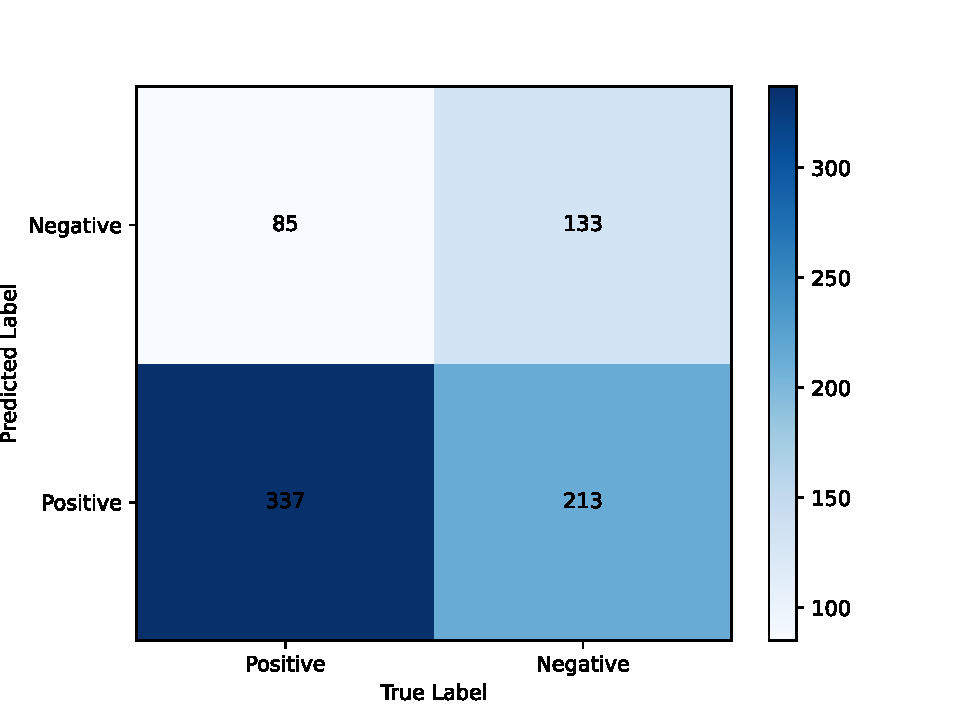
\includegraphics[width=\columnwidth]{img/confusion_matrix_basic.pdf}
  \caption{Confusion matrix for the baseline model, with accuracy of 0.61}
  \label{fig:confusion_matrix_basic}
\end{figure}

The figure~\ref{fig:confusion_matrix_basic} shows the result matrix for one of the basic runs. This particular network leans clearly more towards positive results i.e. images with a smiling person, but this doesn't really help us in optimizing the model, since we are working with a binary classification task with equal proportions of classes.

From the runs we could take an average accuracy of 0.59\% for the basemodel, which is clearly not enough as what was required in the assignment, so we need to apply additional methods to improve the accuracy.

\section{Larger Models}

To find a better model we experimented with larger models by adding non-downsampling blocks after the each side of downsampling block. The base models structure in our syntax is: 1x64 2x32 2x16 1x8. The last layer of each size is always a downsampling layers and the ones before that are non-downsampling layers. The extra layers should be able to capture more features which should enable for better classification. For this experiment we trained for 150 epochs to ensure that the larger models had enough time to learn.

\begin{table}[h!]
\centering
\caption{Training accuracy for different CNN models with Adam optimizer}
\begin{tabular}{|c|c|}
\hline
\textbf{Model} & \textbf{Accuracy}  \\ \hline
2x64 3x64 3x16 2x8 & 0.82 \\ \hline
3x64 4x64 4x16 3x8 & 0.66 \\ \hline
4x64 5x64 5x16 4x8 & 0.63 \\ \hline
2x64 2x64 2x16 1x8 & 0.80 \\ \hline
3x64 2x64 2x16 1x8 & 0.81 \\ \hline
1x64 4x64 4x16 1x8 & 0.83 \\ \hline
3x64 3x64 2x16 1x8 & 0.80 \\ \hline
\end{tabular}
\label{tab:models}
\end{table}

Based on table results shown in table~\ref{tab:models} we can make an hypothesis that increasing the depth in the beginning of the network, where the layers are larger has greatly more effect to classification results.

\section{Hyperparameter Optimization}
This section presents the results of the different tests where we experimented with different hyperparameters.

\subsection{Learning rate}
We tested multiple learning rate for both adam and adamW optimizers. These results are shown in the table~\ref{tab:learningrates}. From the results we can see that the use of adamW didn't really benefit us, not in terms of training time or improved accuracy. This experiment helped us to better narrow down the optimal learning rate for our model.
\begin{table}[h!]
\centering
\caption{Training accuracy for Adam and AdamW optimizers with different learning rates}
\begin{tabular}{|c|c|c|}
\hline
\textbf{Learning Rate} & \textbf{Adam} & \textbf{AdamW} \\ \hline
0.2 & 0.62 & 0.55 \\ \hline
0.02 & 0.56 & 0.56 \\ \hline
0.002 & 0.58 & 0.55 \\ \hline
0.0002 & 0.79 & 0.76 \\ \hline
0.00002 & 0.62 & 0.60 \\ \hline
0.000002 & 0.56 & 0.54 \\ \hline
0.0000002 & 0.58 & 0.52 \\ \hline
0.00000002 & 0.79 & 0.51 \\ \hline
\end{tabular}
\label{tab:learningrates}
\end{table}

We decided to do another experiment with learning rates closer to the values of $0.0002$ which was determined to be best magnitude in the previous experiment. These results are shown in the table~\ref{tab:learningrates2}

\begin{table}[h!]
\centering
\caption{Training accuracy for Adam and AdamW optimizers with different learning rates}
\begin{tabular}{|c|c|c|}
\hline
\textbf{Learning Rate} & \textbf{Adam} & \textbf{AdamW} \\ \hline
0.00005 & 0.63 & 0.61 \\ \hline
0.0001 & 0.66 & 0.70 \\ \hline
0.0003 & 0.64 & 0.62 \\ \hline
0.0005 & 0.62 & 0.62 \\ \hline
0.0007 & 0.61 & 0.58 \\ \hline
\end{tabular}
\label{tab:learningrates2}
\end{table}


From the results we can again see that the choice of optimizer doesn't have much effect in our cage, but it's clear that the learning rate of 0.0001 has produced best results for both of the optimizers. This is still a worse accuracy than what we got with a learning rate of 0.0002.

\subsection{Batch Size}
Batch size is an important factor to consider during the training. Using a large enough batch size will allow the model to be trained faster than with a smaller batch size. Large batch size might also faciliate for some randomness in the optimization preventing the model from getting stuck in local minimas. We tested some possible batch sizes as shown in the table~\ref{tab:batchsizes}.
\begin{table}[h!]
\centering
\caption{Training accuracy for Adam optimizer with different batch sizes}
\begin{tabular}{|c|c|}
\hline
\textbf{Batch Size} & \textbf{Accuracy} \\ \hline
1 & 0.80 \\ \hline
8 & 0.59 \\ \hline
16 & 0.60 \\ \hline
32 & 0.56 \\ \hline
64 & 0.56 \\ \hline
128 & 0.54 \\ \hline
256 & 0.55 \\ \hline
\end{tabular}
\label{tab:batchsizes}
\end{table}

From the results we can see that the batch size didn't have a massive effect on the accuracy. This is most likely since we train for so many epochs. There is a clear outlier in batch size of 1. This might be due to a lucky change in initial weights, but generally larger batch size a used with image classification.

\section{Data augmentation}
We tested the following model: 1x64 3x32 3x16 1x8 with all the datasets described in~\ref{sec:dataaug}. These results are shown in table~\ref{tab:dataaug}.
\begin{table}[h!]
\centering
\caption{Training accuracy for Adam optimizer with the specified datasets}
\begin{tabular}{|c|c|}
\hline
\textbf{Dataset} & \textbf{Accuracy} \\ \hline
Base & 0.85 \\ \hline
Grayscale & 0.75 \\ \hline
Augmented & 0.87  \\ \hline
Augmented Grayscale & 0.83  \\ \hline
\end{tabular}
\label{tab:dataaug}
\end{table}

From the results we can conclude that our hypothesis about grayscale leaving more space for parameters to find features was not correct, since the grayscale datasets performed clearly worse then the color sets. We can also see that data augmentaion improved our accuracy a bit.

We also experimented with noise as mentioned in section~\ref{sec:noise}, by adding random gaussian noise to input dynamically before the forward pass. This didn't clearly benefit our model's performance in any way, rather it lowered the accuracy regardless of the other parameters and it slowed down the training by a small factor. The likely reason is that the amount of noise we are adding is too much or that the image are already noisy and adding more noise makes the task significantly harder. Either way we didn't have enough time to quantify the reason or do more indepth testing for this feature.

\section{The Final Model}
After all the experimentation we settled on the following model for our training: 3x64 3x32 2x16 1x8, and we trained for 200 epochs, with the augmented color images, without noise, with a learning rate of $0.0002$ using the Adam optimizer, with batches of 32. On M1 macbook this took around 90 minutes with GPU acceleration via the MPS backend.

Since we were limited on time and processing hardware we cannot be sure that this given model is the most performant model that we could have achieved. In our testing the model achieved an accuracy of: 88\% and was sufficiently accurate and fast when we tested it in the completed system.

\begin{figure}
  \centering
  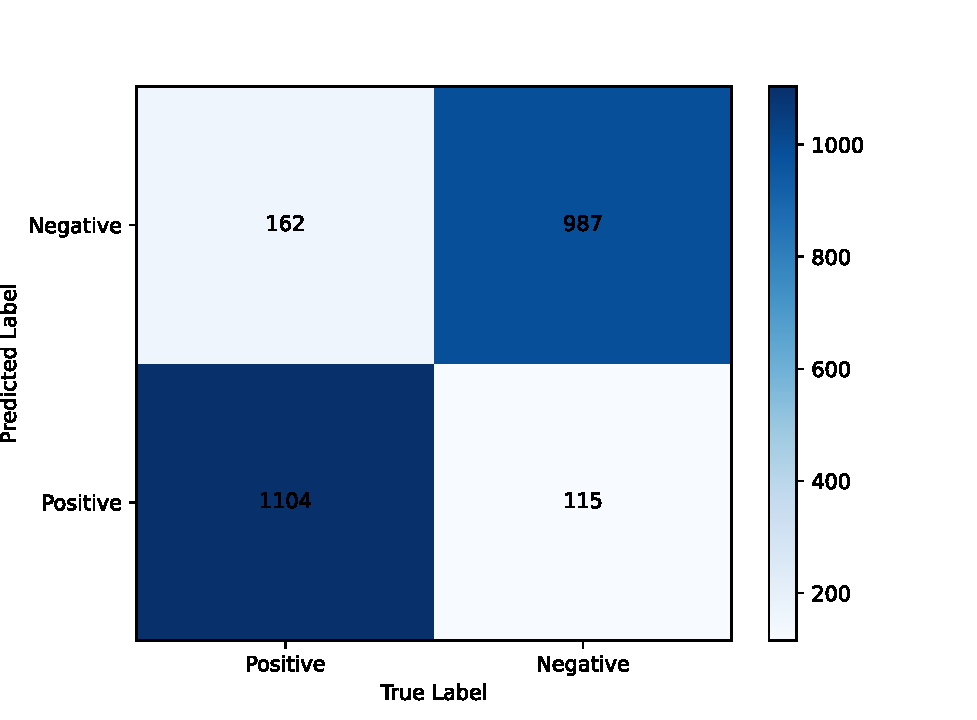
\includegraphics[width=\columnwidth]{img/confusion_matrix_best.pdf}
  \caption{Confusion matrix for the best performing model, with augmented dataset of 2368 images}
  \label{fig:confusion_matrix_best}
\end{figure}

\begin{figure}
  \centering
  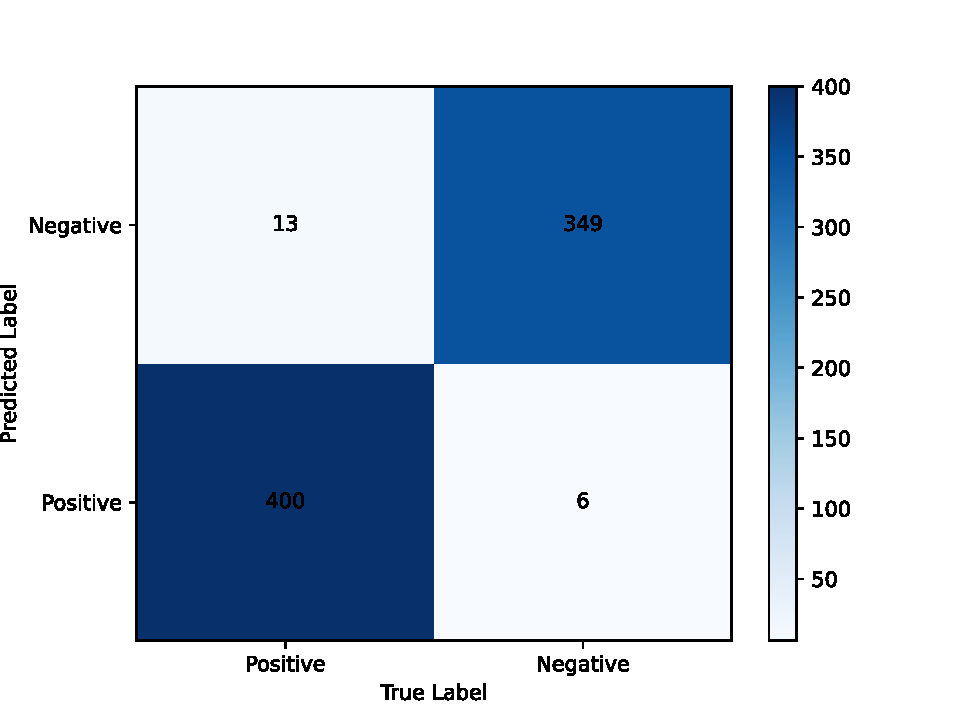
\includegraphics[width=\columnwidth]{img/confusion_matrix_small.pdf}
  \caption{Confusion matrix for the best performing model, with non-augmented dataset of 800 images}
  \label{fig:confusion_matrix_small}
\end{figure}


The figure~\ref{fig:confusion_matrix_best} shows the confusion matrix for the final model.

Since the model was trained with augmented data we also tested the accuracy for the non-augmented data set where we got a extreamly good accuracy score of 97.53\%. Figure~\ref{fig:confusion_matrix_small} shows the confusion matrix for this test. From this matrix we can still see that the model fails slightly more with smiling images that it predicts to be non-smiling.

\section{Smile Detection}
When we initially tested our smile detection system with real-time video feed, the results did not totally meet our expectations, despite achieving a training model accuracy of over 85\%. After further research, we found a potential problem in the Region of Interest (ROI) around detected faces. In the training images used for the model, the images were much farther away taken (with hair and shoulders included), compared to our face ROI, which is capped only on the face.  

To solve this problem, we added a "scalar factor" parameter, that allows us to dynamically scale the ROI. We found that by increasing the face ROI to twice the size of the original ROI obtained from the Cascade classifier, our smile recognition system improved significantly. Figures~\ref{fig:smiling} and~\ref{fig:not_smiling} in the Appendix 1 show positive and negative prediction results, from a live feed capture. Appendix 2 presents examples images for the 4 bayesian prediction results as predicted by the model.


\chapter{Conclusions}
\label{ch:conclusions}

In this assignment, we familiarized ourselves with machine learning in particular deep learning methods. Our goal was to create a smile detector using deep network and deploy that for real-time execution. 

First we implemented and trained the baseline model as per assignment instructions, with Pytorch. We then evaluated the baseline's performance, and chose methods to improve the classification accuracy. Our main methods for increasing the model's accuracy were data augmentation, increasing the size of the network and hyperparameter tuning. With these methods we successfully increased the accuracy over the required threshold of 85\% up to 88\%.

Second, we integrated the model with the OpenCV library to classify smiles from a live video feed. However, after the integration, our smile detection program didn't work as well as we hoped. To remedy this, we scaled the face Region of Interest (ROI) to cover a wider area. This adjustment led to significant improvements in the interface and we were satisfied with the result.

In summary, the goal of this assignment was to build a program that could classify from live video feed if the person in the video is smiling or not, with an accuracy of at least 85\%. The program we built during this project satisfies these requirements.
%
% The bibliography, i.e the list of references
%
\newpage

\printbibliography[title=References]
\addcontentsline{toc}{chapter}{References}

\appendix
\pagestyle{headings}

%
% a) Not-so-handy way, but at least it works
%
\def\appA{APPENDIX 1 Live feed prediction examples} % Define the name and numbering manually
\chapter*{\appA}                       % Create chapter heading
\markboth{\appA}{\appA}                % Set page header
\addcontentsline{toc}{chapter}{\appA}  % Include this in TOC
% Note that \label does not work with unnumbered chapter
Here are presented screencaptures from smile detection functionality when used with a webcam.
%\section{Live feed predictions}\label{sec:app_live}
\begin{figure}[hbt!]
  \centering
  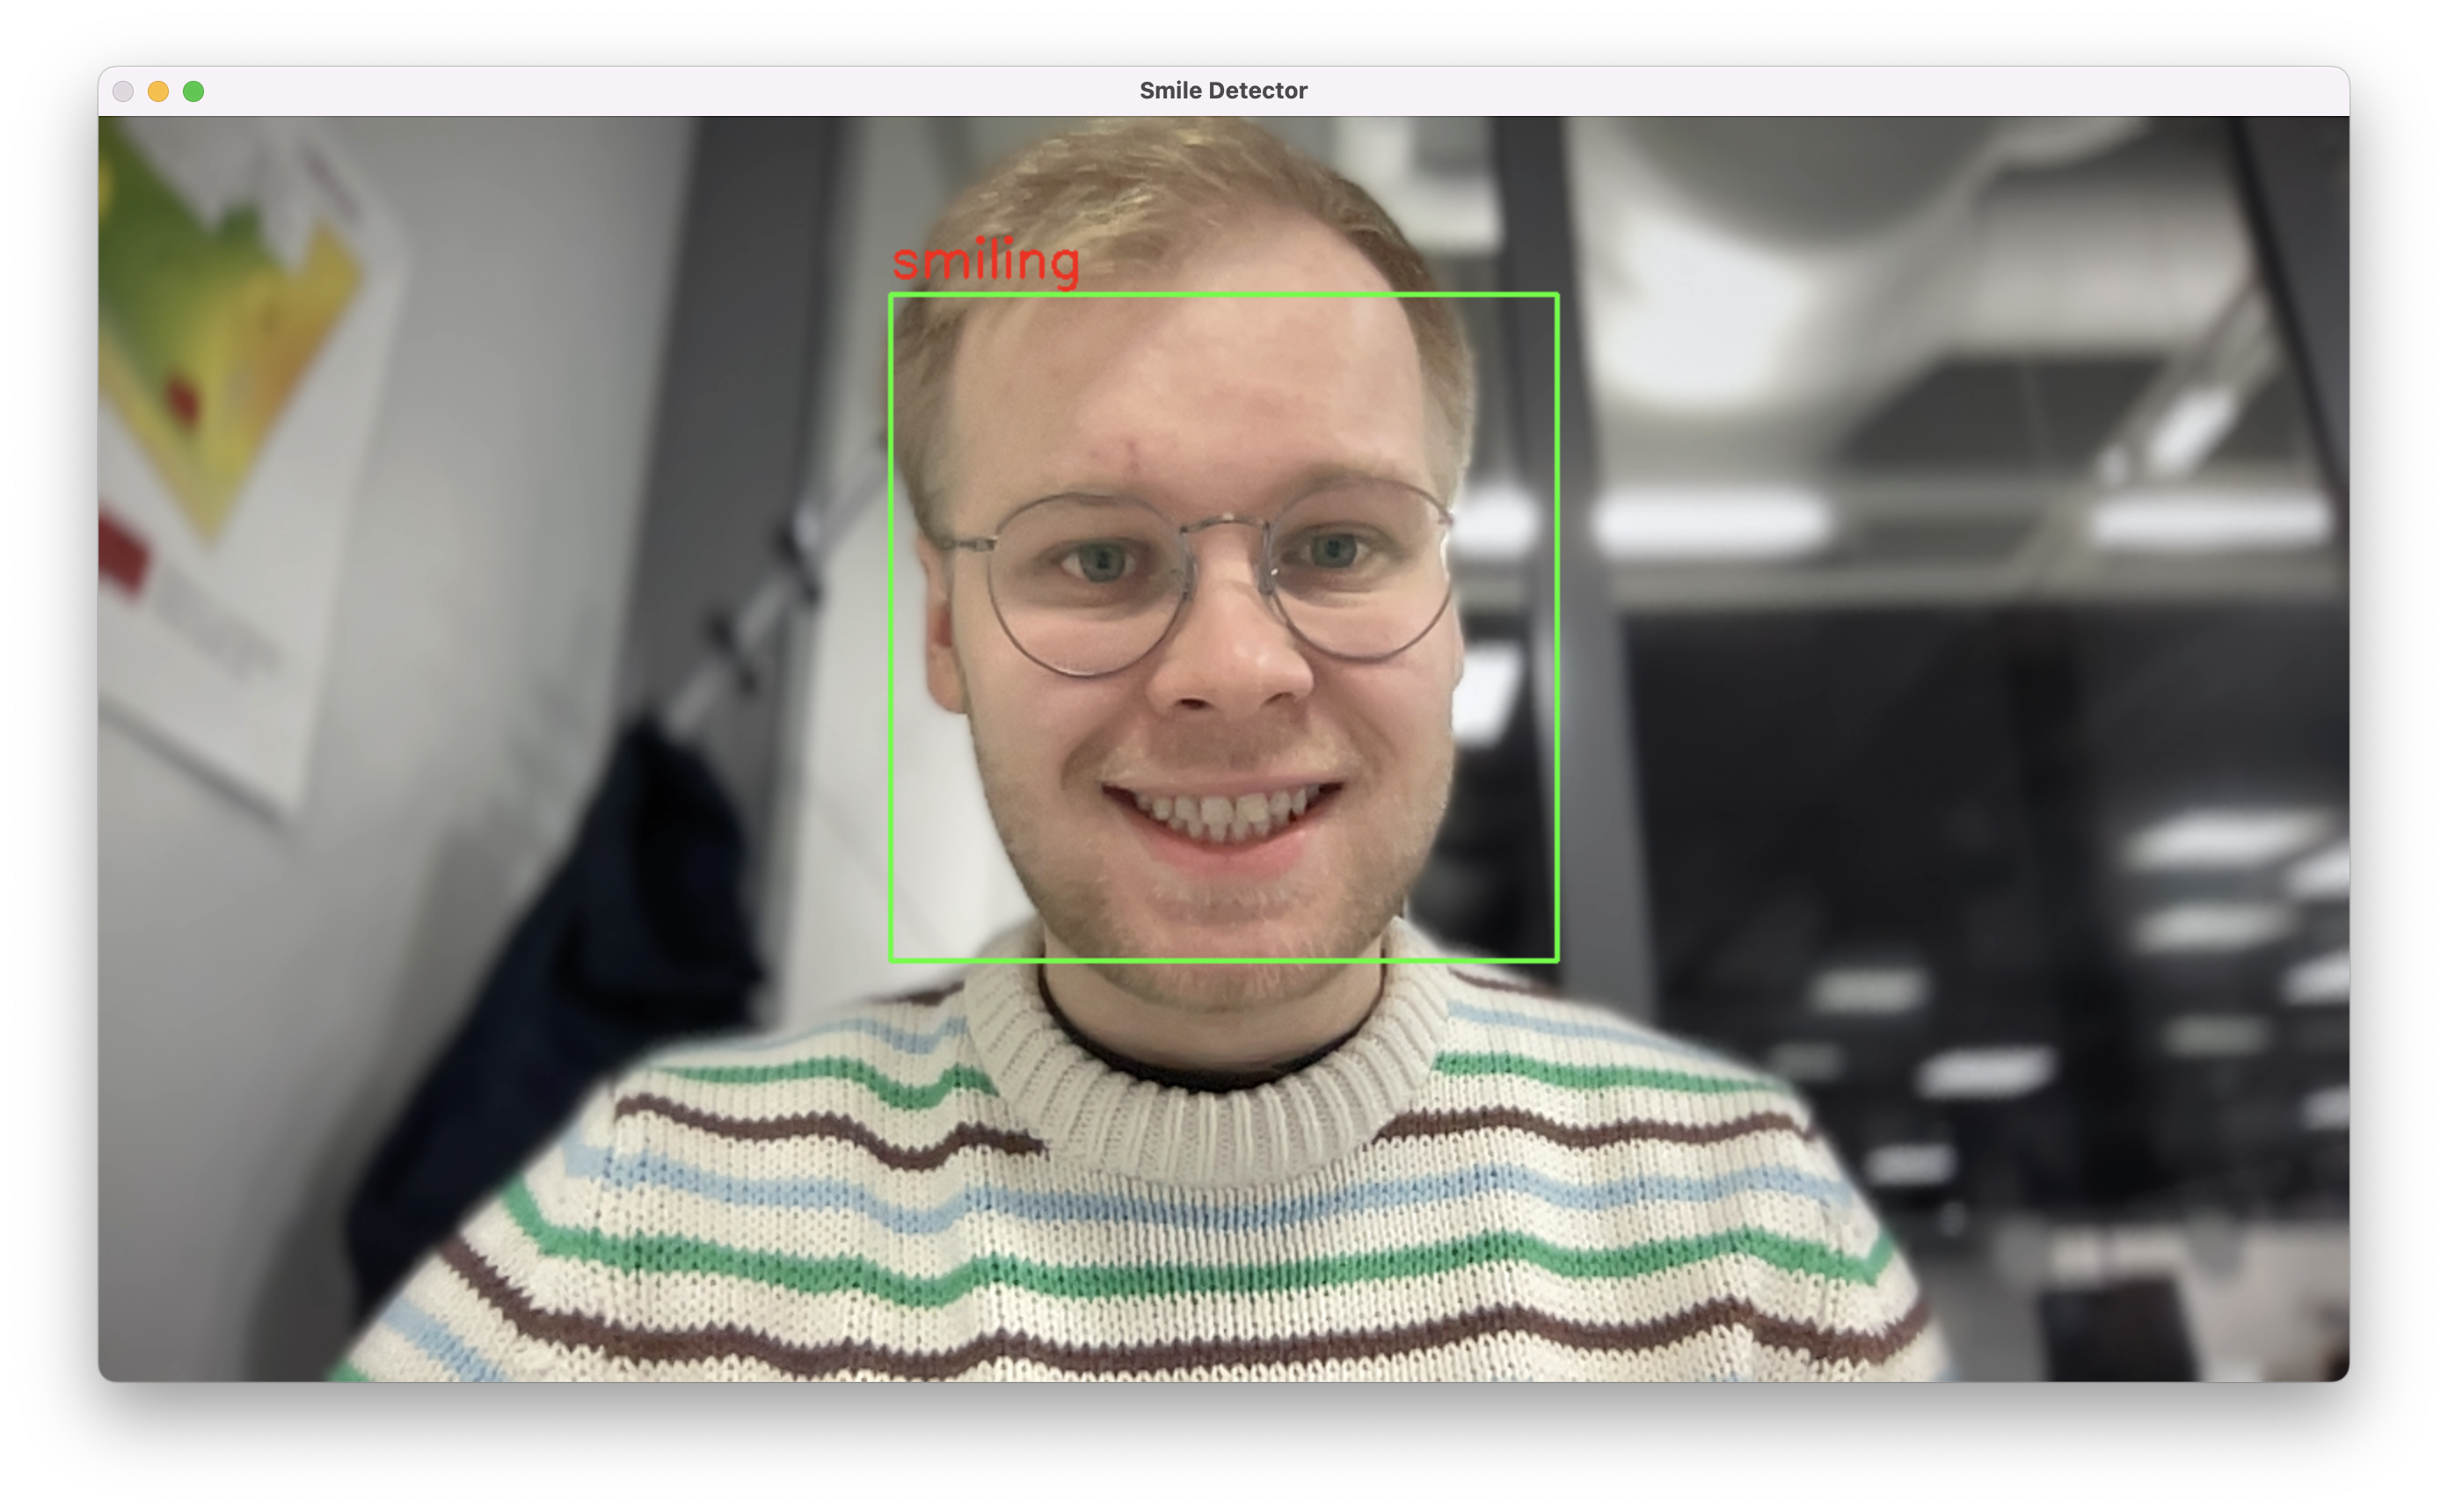
\includegraphics[width=\columnwidth]{img/smiling.png}
  \caption{Positive prediction from a live feed capture}
  \label{fig:smiling}
\end{figure}

\begin{figure}[hbt!]
  \centering
  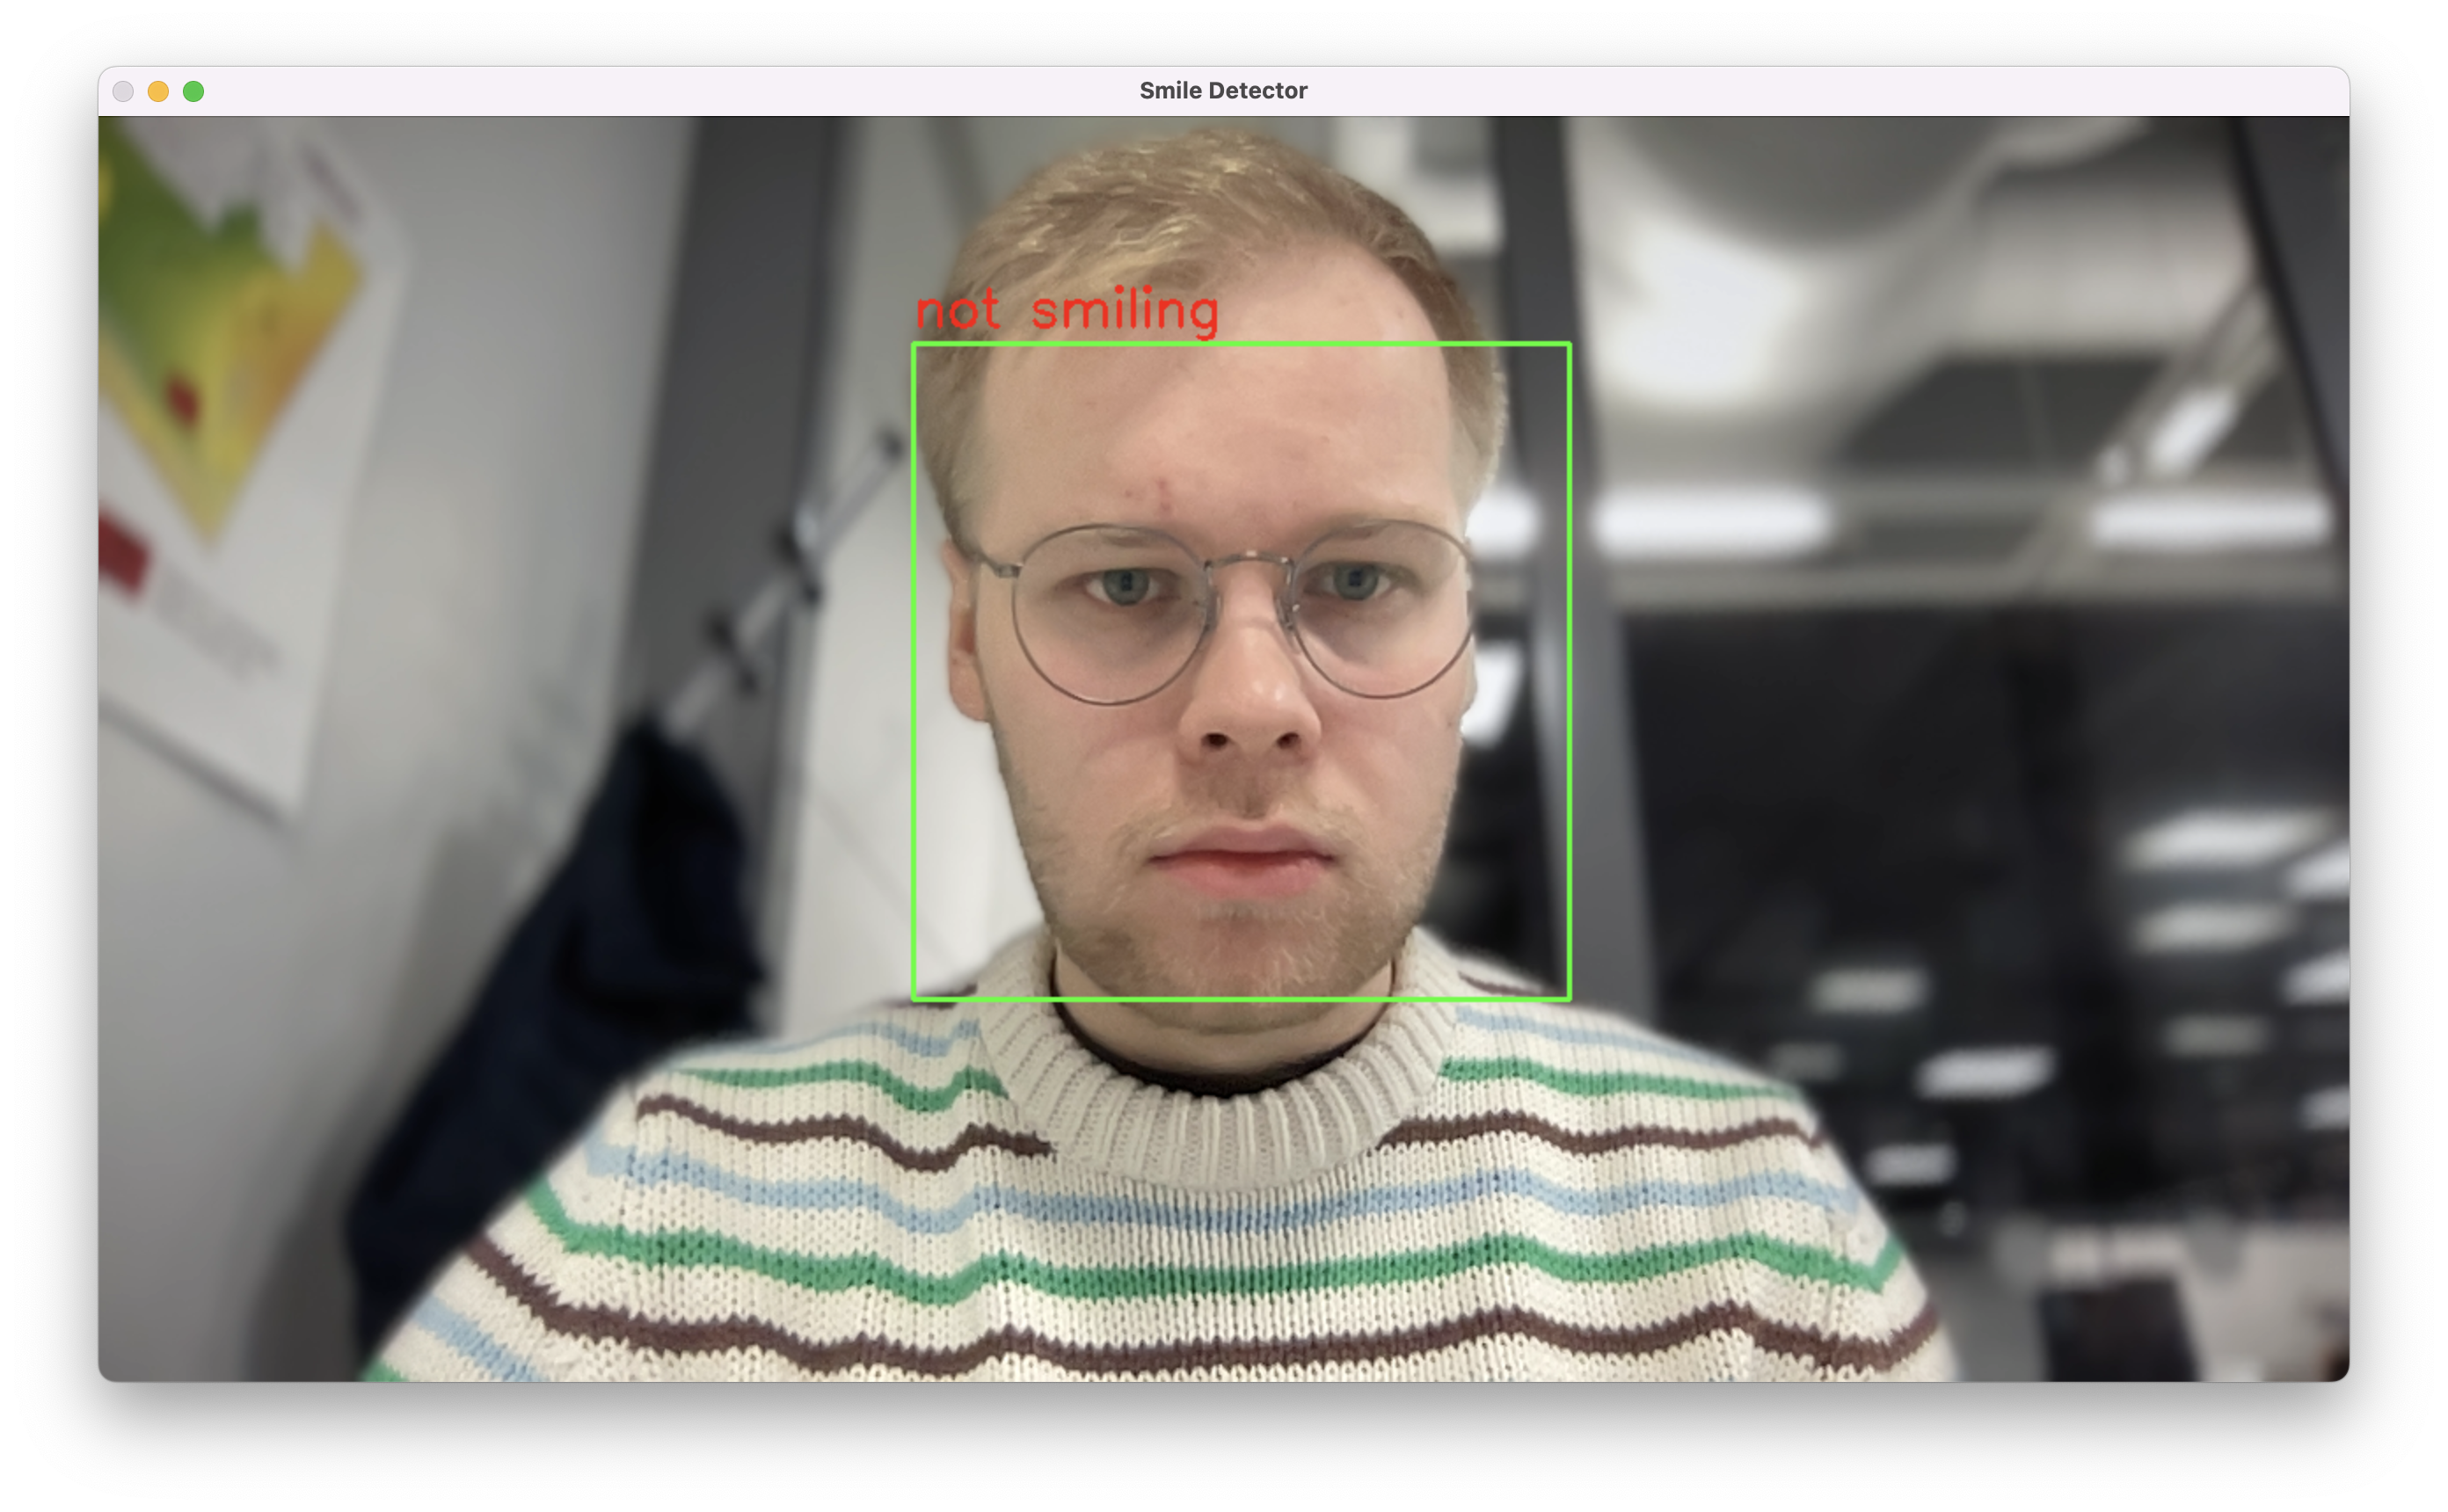
\includegraphics[width=\columnwidth]{img/not_smiling.png}
  \caption{Negative prediction from a live feed capture}
  \label{fig:not_smiling}
\end{figure}

\def\appB{APPENDIX 2 Bayesian predictions results from testing} % Define the name and numbering manually
\chapter*{\appB}                       % Create chapter heading
\markboth{\appB}{\appB}                % Set page header
\addcontentsline{toc}{chapter}{\appB}  % Include this in TOC

%\section{Predictions results from testing}\label{sec:app_bayes}
Here are presented samples obtained during model test run for each of the bayesian prediction result classes. Figure~\ref{fig:tps} shows 4 true positive samples, figure~\ref{fig:tns} shows true negatives, figure\ref{fig:fps} shows false positives and figure~\ref{fig:fns} shows false negatives.
\begin{figure}[hbt!]
  \centering
  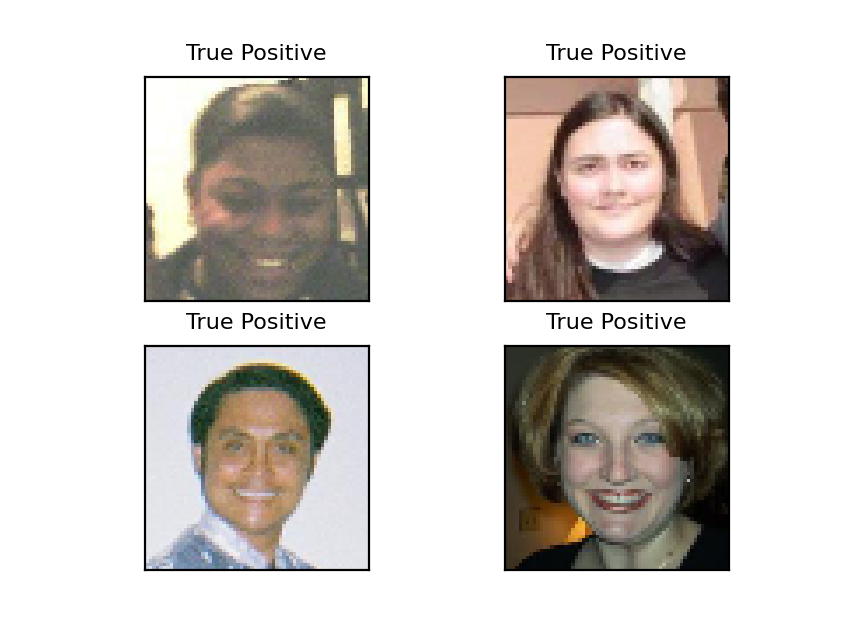
\includegraphics[width=0.8\columnwidth]{img/tps.png}
  \caption{True positive samples predicted by the best performing model}
  \label{fig:tps}
\end{figure}

\begin{figure}[hbt!]
  \centering
  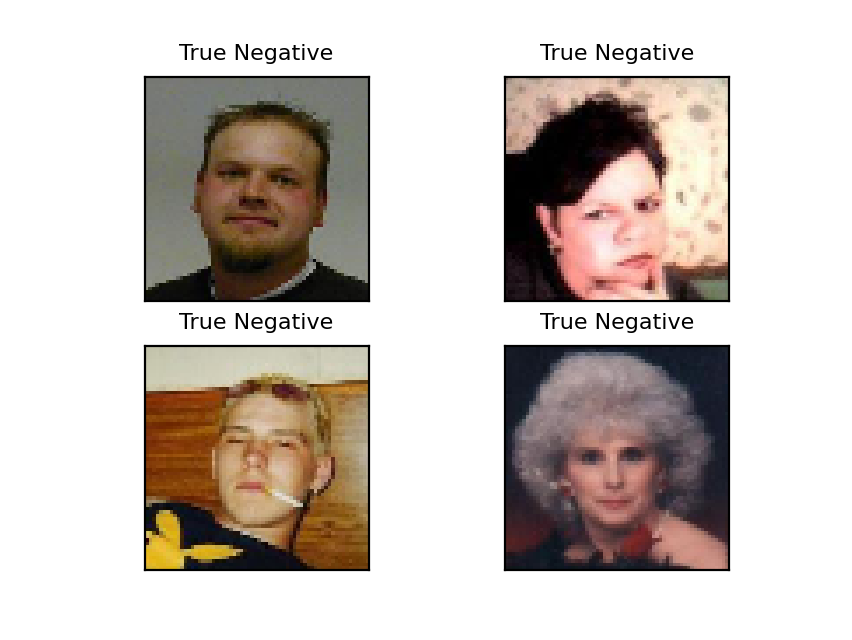
\includegraphics[width=0.8\columnwidth]{img/tns.png}
  \caption{True negative samples predicted by the best performing model}
  \label{fig:tns}
\end{figure}

\begin{figure}[hbt!]
  \centering
  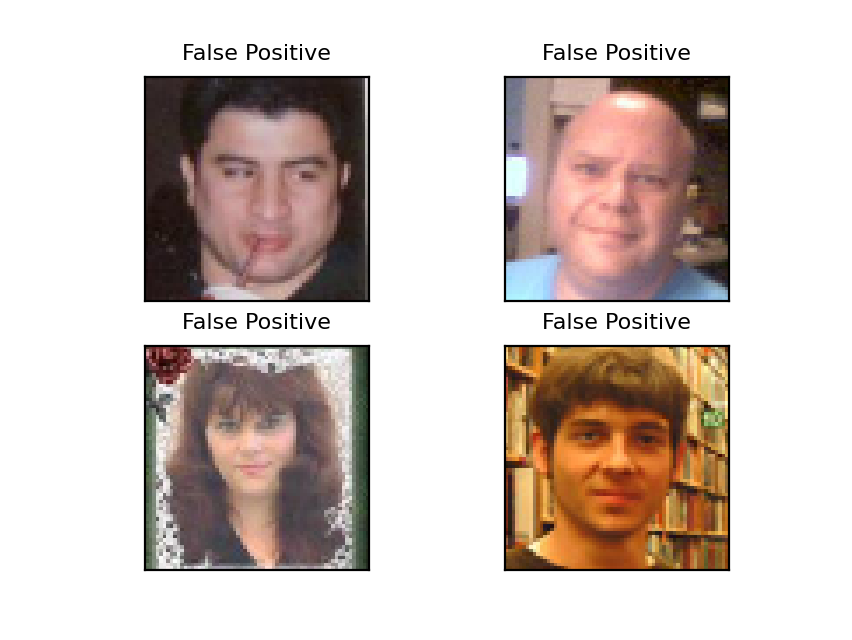
\includegraphics[width=0.8\columnwidth]{img/fps.png}
  \caption{False positive samples predicted by the best performing model}
  \label{fig:fps}
\end{figure}

\begin{figure}[hbt!]
  \centering
  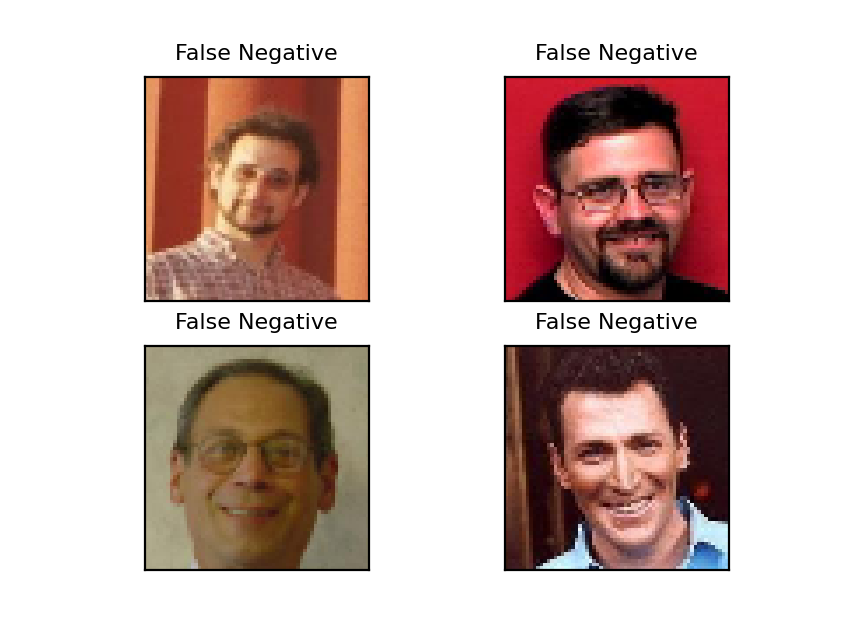
\includegraphics[width=0.8\columnwidth]{img/fns.png}
  \caption{False negative samples predicted by the best performing model}
  \label{fig:fns}
\end{figure}

\def\appC{APPENDIX 3 Running the code} % Define the name and numbering manually
\chapter*{\appC}                       % Create chapter heading
\markboth{\appC}{\appC}                % Set page header
\addcontentsline{toc}{chapter}{\appC}  % Include this in TOC

%\section{Running the code}
The instructions to run the program are displayed in the README.md file, which was hopefully included along side this document.



\end{document}

